% $Header: /cvsroot/latex-beamer/latex-beamer/solutions/generic-talks/generic-ornate-15min-45min.en.tex,v 1.5 2007/01/28 20:48:23 tantau Exp $

\documentclass[12pt]{beamer}
%\documentclass[12pt,handout]{beamer}

% This file is a solution template for:

% - Giving a talk on some subject.
% - The talk is between 15min and 45min long.
% - Style is ornate.



% Copyright 2004 by Till Tantau <tantau@users.sourceforge.net>.
%
% In principle, this file can be redistributed and/or modified under
% the terms of the GNU Public License, version 2.
%
% However, this file is supposed to be a template to be modified
% for your own needs. For this reason, if you use this file as a
% template and not specifically distribute it as part of a another
% package/program, I grant the extra permission to freely copy and
% modify this file as you see fit and even to delete this copyright
% notice.


\mode<presentation>
{
  \usetheme{default}
  % or ...

  \setbeamercovered{transparent}
  % or whatever (possibly just delete it)
}
\setbeamertemplate{navigation symbols}{}%remove navigation symbols


\usepackage[english]{babel}
% or whatever

\usepackage[latin1]{inputenc}
% or whatever

\usepackage{times}
\usepackage{sansmathfonts}
\usepackage[T1]{fontenc}
% Or whatever. Note that the encoding and the font should match. If T1
% does not look nice, try deleting the line with the fontenc.


\title%[Short Paper Title] % (optional, use only with long paper titles)
{}

\subtitle
{} % (optional)

\author%[Author, Another] (optional, use only with lots of authors)
{Ben Holder}%{F.~Author\inst{1} \and S.~Another\inst{2}}
% - Use the \inst{?} command only if the authors have different
%   affiliation.

%\institute[Universities of Somewhere and Elsewhere] % (optional, but mostly needed)
%{
%  \inst{1}%
%  Department of Computer Science\\
%  University of Somewhere
%  \and
%  \inst{2}%
%  Department of Theoretical Philosophy\\
%  University of Elsewhere}
%% - Use the \inst command only if there are several affiliations.
%% - Keep it simple, no one is interested in your street address.

\date%[Short Occasion] % (optional)
{}

\subject{Talks}
% This is only inserted into the PDF information catalog. Can be left
% out.



% If you have a file called "university-logo-filename.xxx", where xxx
% is a graphic format that can be processed by latex or pdflatex,
% resp., then you can add a logo as follows:

% \pgfdeclareimage[height=0.5cm]{university-logo}{university-logo-filename}
% \logo{\pgfuseimage{university-logo}}



% Delete this, if you do not want the table of contents to pop up at
% the beginning of each subsection:
%\AtBeginSubsection[]
%{
%  \begin{frame}<beamer>{Outline}
%    \tableofcontents[currentsection,currentsubsection]
%  \end{frame}
%}


% If you wish to uncover everything in a step-wise fashion, uncomment
% the following command:

%\beamerdefaultoverlayspecification{<+->}

\usepackage{enumerate}
\usepackage{amsmath}
\usepackage{amssymb}
\usepackage[amssymb]{SIunits}
\usepackage{url}
\usepackage{hyperref}
\usepackage[normalem]{ulem}


\setbeamercovered{invisible}

\hypersetup{
    colorlinks=true,     % false: boxed links; true: colored links
    linkcolor=red,       % color of internal links
    citecolor=blue,      % color of links to bibliography
    filecolor=blue,      % color of file links
    urlcolor=blue        % color of external links
}


\begin{document}

%\begin{frame}
%  \titlepage
%\end{frame}

%%%%%%%%%%%%%%%%%%%%%%%%%%%%%%%%%%%%%%
\begin{frame}{Announcements}
	%
	\begin{itemize}
	\addtolength{\itemsep}{0.5\baselineskip}
	\item Catching up on grading: come ask me if you have questions.
	\item I will not have my Wed (2--3pm) office hour this week; email me to meet at another time.
	\item \underline{Schedule}:
		%
		\begin{itemize}
		\item[]{\bf Today (Follow-up)}: Equilibrium temperature without atmosphere
		\item[]{\bf Today (New)}: Atmosphere and Greenhouse Effect (week 1)
		\item[]{\bf Tomorrow (Lab)}: ``feel the sun on your face (no one else can do it for you)''
		\item[]{\bf Thursday (Discussion)}: Calculating equilbrium temperatures with atmospheres
		\item Next Week: Greenhouse Effect II
		\end{itemize}
		%
	\end{itemize}

\end{frame}
%%%%%%%%%%%%%%%%%%%%%%%%%%%%%%%%%%%%%%
\begin{frame}{Today's Reading Quiz (3 min)}


	
\vspace{1cm}

On your own sheet of paper\ldots

\vspace{0.5cm}

{\bf What are the key physical characteristics of our atmosphere (related to EM radiation, transparency, and opaqueness)  that cause the ``greenhouse effect''?}

\vspace{0.5cm}

Turn in to Blackboard as scanned pdf (or image is fine).

\end{frame}
%%%%%%%%%%%%%%%%%%%%%%%%%%%%%%%%%%%%%%
\begin{frame}{Key information and equations from last week}

\underline{Wien's Law (wavelength of BB peak)}
\begin{equation*}
\lambda_\text{peak} = \frac{\unit{2900}{\micro\meter \cdot \kelvin}}{T}
\end{equation*}


\underline{Stefan-Boltzmann Law (total flux output)}
\begin{equation*}
F = \left( 6 \times 10^{-8} \, \frac{\text{J}/\text{s}}{\text{m}^2 \cdot \text{K}}\right) T^4
\end{equation*}


\underline{Peak value of  ``Spectral Flux'' BB curve}
\begin{equation*}
F_\lambda = \frac{F}{1.5 \times \lambda_\text{peak}}
\end{equation*}

\begin{center}
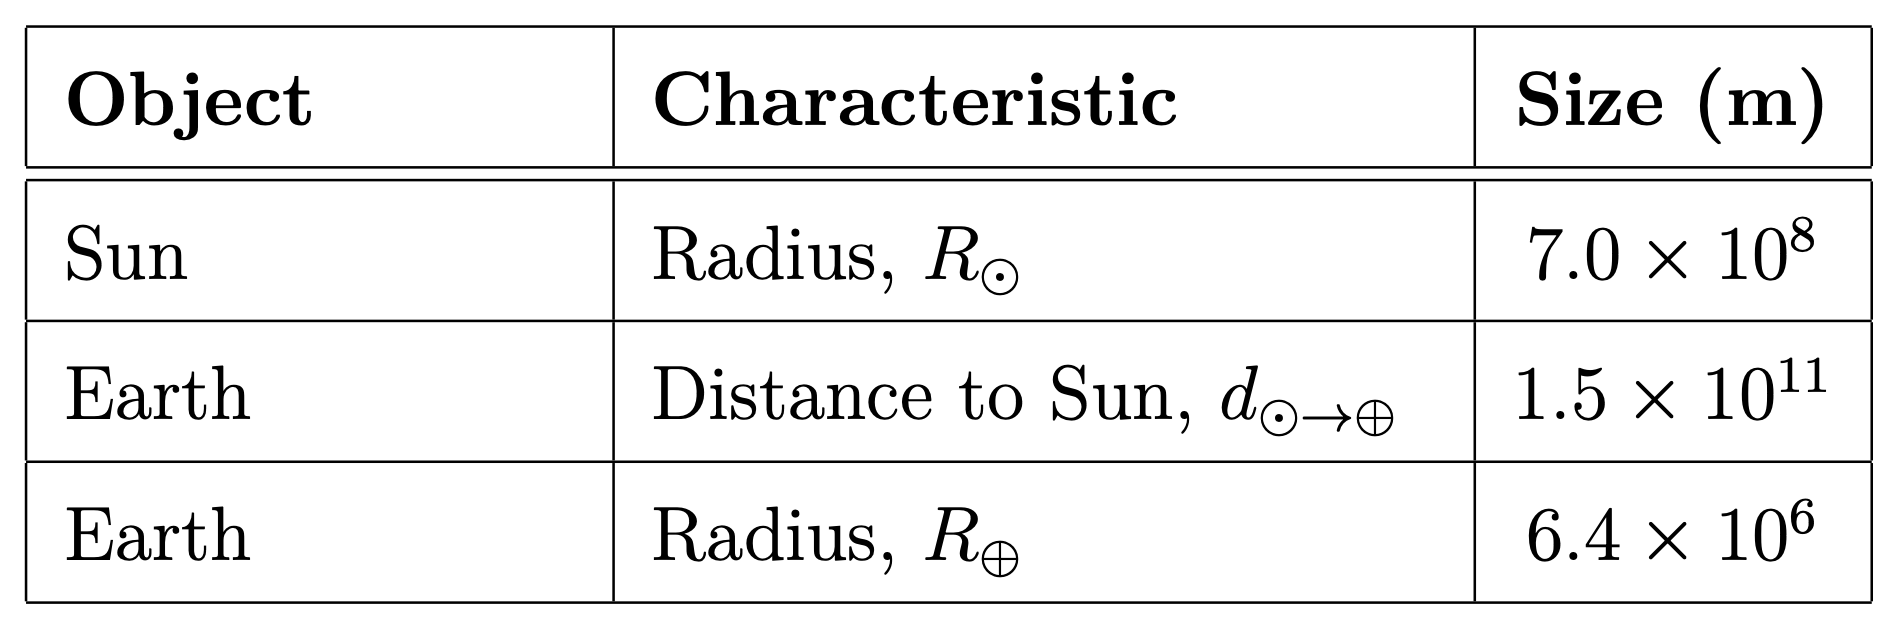
\includegraphics[width=0.7\textwidth]{images/astronomical-distances}
\end{center}

\end{frame}
%%%%%%%%%%%%%%%%%%%%%%%%%%%%%%%%%%%%%%
\begin{frame}{Questions 2--3 --- Overview}

\begin{itemize}
\item In Question 2, we wish to find the average solar flux (power per area, in $\frac{\text{J}/\text{s}}{\text{m}^2}$) reaching the Earth's surface, call it $F_\text{from Sun}$.
\item To calculate equilibrium temperature (Question 3), we assume that:
	%
	\begin{equation*}
	\begin{split}
	F_\text{from Sun} &= F_\text{of Earth}\\
	F_\text{from Sun} &= F_\text{of Earth}(T_\text{Earth})\\
	\end{split}
	\end{equation*}
	%
where the flux ``from Earth'' is its output power per area due to {\em being a blackbody radiator}.  
\item The temperature of the Earth, $T_\text{Earth}$, is an unknown at this point (that's what we want to find), but the dependence of the Earth's flux on temperature is just the Stefan-Boltzmann Law:
	%
	\begin{equation*}
	F_\text{of Earth} (T_\text{Earth}) = \left( 6 \times 10^{-8} \, \frac{\text{J}/\text{s}}{\text{m}^2 \cdot \text{K}}\right) T_\text{Earth}^4
	\end{equation*}

\end{itemize}

\end{frame}
%%%%%%%%%%%%%%%%%%%%%%%%%%%%%%%%%%%%%%
\begin{frame}{Question 2(a) --- Finding Power of the Sun}

The sun is a blackbody radiator, emitting flux (power per area) according to the Stefan-Boltzmann Law:
%
\begin{equation*}
F = \left( 6 \times 10^{-8} \, \frac{\text{J}/\text{s}}{\text{m}^2 \cdot \text{K}}\right) T^4
\end{equation*}
%
It's total power output is that flux multiplied by its total surface area (as a sphere, $A = 4 \pi R^2$).

\vspace{5cm}

\end{frame}
%%%%%%%%%%%%%%%%%%%%%%%%%%%%%%%%%%%%%%
\begin{frame}{Question 2(b) --- Finding the ``Solar Constant''}


\begin{columns}[T]
\column{0.55\textwidth}

The so-called ``Solar Constant'', $S$, is the flux (in $\frac{\text{J}/\text{s}}{\text{m}^2}$) of the Sun at the position of the Earth in orbit.  This is approximately what someone at the Equator would receive if there were no clouds.

\column{0.35\textwidth}
\vspace{0pt}
\begin{center}
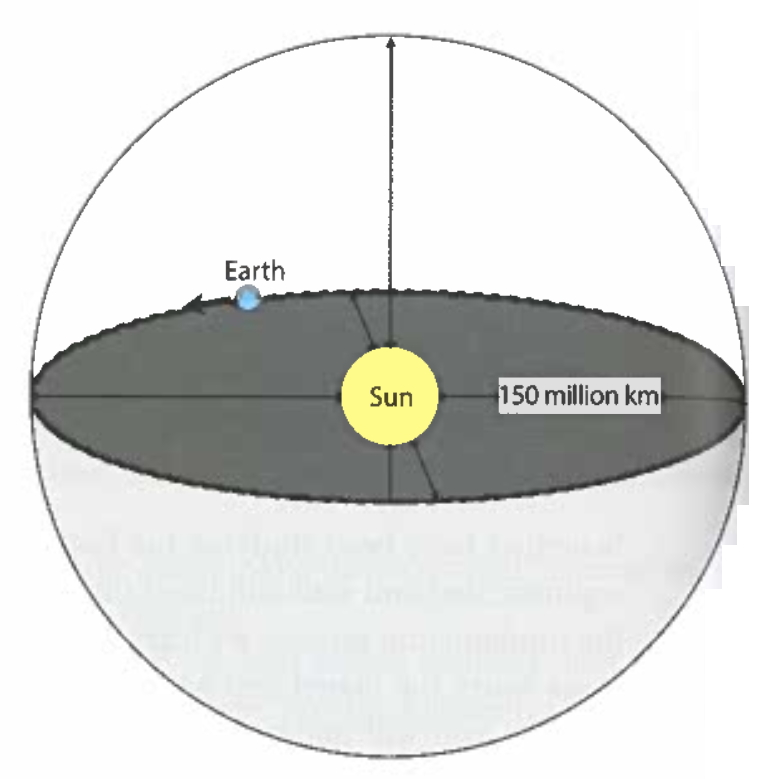
\includegraphics[width=0.9\textwidth]{images/dessler_4-1}
\end{center}
\end{columns}

\vspace{5cm}

\end{frame}
%%%%%%%%%%%%%%%%%%%%%%%%%%%%%%%%%%%%%%
\begin{frame}{Question 2(c) --- Finding avg flux at the surface}


\begin{columns}[T]
\column{0.53\textwidth}
We obtain an average solar flux (power per area) at the Earth's surface by (i) calculating the total power ``caught'' by the Earth (see image at right), and

\column{0.45\textwidth}
\vspace{0pt}
\begin{center}
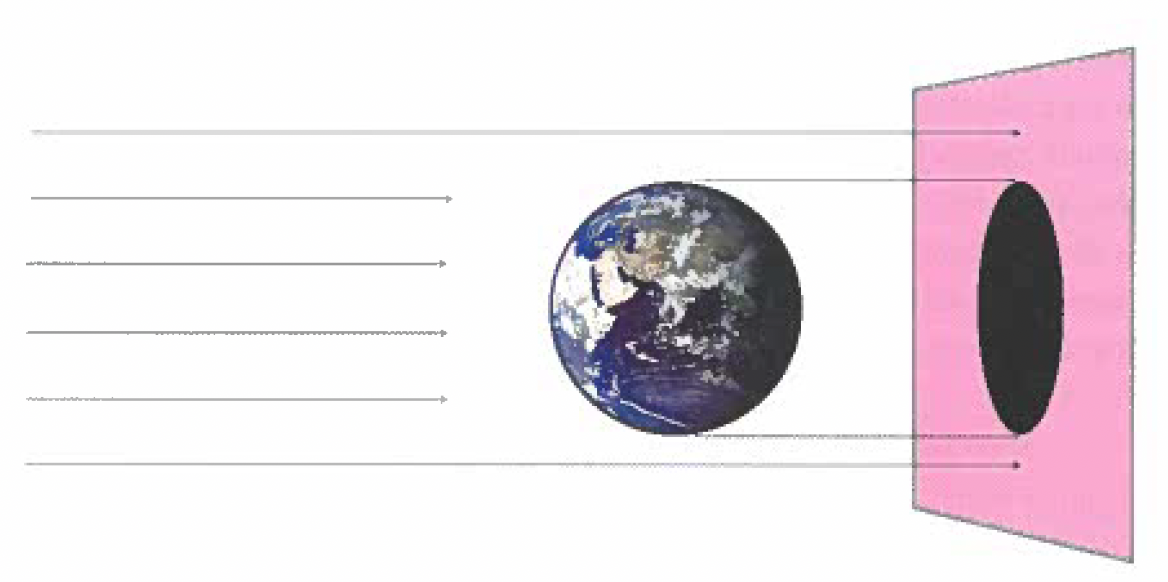
\includegraphics[width=\textwidth]{images/dessler_4-2}
\end{center}
\end{columns}
\vspace{-0.25cm}
\hspace{-0.5cm} (ii) dividing that power over the Earth's surface evenly.


\vspace{7cm}


\end{frame}
%%%%%%%%%%%%%%%%%%%%%%%%%%%%%%%%%%%%%%
\begin{frame}{Question 2(d) --- Accounting for Clouds and Ice}

A large fraction of the Sun's power is reflected back into space by the Earth.  The name of this reflective fraction is the ``albedo'' and is given by the Greek letter  alpha, $\alpha$.  We estimate that $\alpha \approx 0.3 = 30\%$. Therefore the actual average solar flux at the surface, our $F_\text{from Sun}$, is \ldots


\vspace{5.5cm}

{\tiny Q: How do we actually measure the albedo? A: Earthshine on the Moon! (obviously)}
\end{frame}
%%%%%%%%%%%%%%%%%%%%%%%%%%%%%%%%%%%%%%
\begin{frame}{Question 3 --- Estimating $T_\text{Earth}$}
	
	\begin{enumerate}[(a)]
	\item Draw an energy flow diagram for the Sun-Earth system.
	\item If we assume the Earth is in equilibrium (``total'' energy is constant, so $T$ is constant), what equation do we obtain?  What is the equilibrium value of the Earth's temperature?
	\item Is this answer correct?  Why or why not?
	\end{enumerate}
	


\vspace{7cm}

\end{frame}
%%%%%%%%%%%%%%%%%%%%%%%%%%%%%%%%%%%%%%
\begin{frame}{Now, what about with an atmosphere?}

The details of our atmosphere are approximately:
	%
	\begin{itemize}
	\item The atmosphere is {\em transparent} to the Sun's visible light. (So our prior calculations are unchanged)
	\item The atmosphere is {\em opaque} to (far) infrared light, like the Earth's thermal radiation at $\sim15\degree$C.
	\item The atmosphere is a blackbody, radiating up and down.
	\end{itemize}
	%
Let's make an energy flow diagram\ldots

\vspace{7cm}

\end{frame}
%%%%%%%%%%%%%%%%%%%%%%%%%%%%%%%%%%%%%%
\end{document}
